%% LC n -> see Latex Companion p. n

%% --------------------------------------------------------------------
%% Various Packages
%% --------------------------------------------------------------------

\usepackage{savesym}
%\usepackage{yfonts}             %% initials, LC 183
\usepackage{amsmath}
\usepackage{amsfonts} % AdM
\usepackage{amssymb}
%\usepackage{wraptable}
\usepackage{wrapfig}
\usepackage{multirow}
%\usepackage{amscd}
%\usepackage{pifont}             %% PostScript symbols, LC 337
%\usepackage{textcomp}           %% Trademark sign

%\usepackage{theorem}            %% environment, LC 251
%\usepackage{fancybox}           %% fancy frames, LC 278
%\usepackage{float}              %% new float types, LC 146

\usepackage{xspace} % AdM       %% smart space, LC 50
\usepackage{placeins}
\usepackage{tabularx}           %% automatic col widths, LC 113
% \usepackage[hidelinks]{hyperref}
\usepackage{pdflscape}



%% --------------------------------------------------------------------
%% Publication quality tables in LaTeX
%% --------------------------------------------------------------------
%% some additional commands to enhance the quality of tables in LaTeX.
%\usepackage{longtable}          %% multi page tables, LC 122
\usepackage{booktabs}
\renewcommand{\heavyrulewidth}{0.08em}
\renewcommand{\lightrulewidth}{0.05em}
\renewcommand{\cmidrulewidth}{0.03em}
\renewcommand{\defaultaddspace}{0.25em}

%% --------------------------------------------------------------------
%% Subfigures
%% --------------------------------------------------------------------
\usepackage[sl]{subfigure}       %% (with slanted labels) LC 152
% all below defaults to 10pt, see package subfigure
\ifthenelse{\boolean{Afive}}{
  \renewcommand{\subfigtopskip}{0pt}
  \renewcommand{\subfigbottomskip}{6pt}
  \renewcommand{\subfigcapskip}{3pt}
  \renewcommand{\subfigcapmargin}{4pt}
}{
  \renewcommand{\subfigtopskip}{6pt}
  \renewcommand{\subfigbottomskip}{12pt}
  \renewcommand{\subfigcapskip}{2pt}
  \renewcommand{\subfigcapmargin}{6pt}
}

%% --------------------------------------------------------------------
%% Definitions for theorem package
%% --------------------------------------------------------------------
%\theoremstyle{break}
%\theoremheaderfont{\scshape}
%\theorembodyfont{\normalfont}                   %% See LaTeX companion p. 171
%\newtheorem{Def}{Definition}
%\newtheorem{Satz}{Satz}

% {\theoremstyle{plain}
% \theoremheaderfont{\normalfont \bfseries}
% \theorembodyfont{\normalfont}
% \newtheorem{Def}{Definition}[chapter]
% \newtheorem{Satz}{Satz}}

% {\theoremstyle{plain}
% \theoremheaderfont{\normalfont \bfseries}
% \theorembodyfont{\itshape}
% \newtheorem{Theorem}{Theorem}[chapter]
% }

%% --------------------------------------------------------------------
%% Inverse search
%% --------------------------------------------------------------------
% \usepackage[active]{srcltx}

%% --------------------------------------------------------------------
%% Unused Packages
%% --------------------------------------------------------------------
\usepackage{times}                                 %% Schriftart auswaehlen
%%\usepackage{times}                                 %% Schriftart auswaehlen
%%\usepackage[]{pslat                                %% Schriftart auswaehlen
%%\usepackage[]{rawfos}                              %% Schriftart auswaehlen
%%\usepackage{a4wide}
%%\usepackage{verbatim}
%%\usepackage{afterpage}
%%\usepackage{multicol}
%%\usepackage{exscale}
%%\usepackage{supertabular}                             %% See Companion p. 119
%%\usepackage[figuresright]{rotating}   %% See Companion p. 320, Problem with pdf
%%\usepackage{enumerate}                                %% See Companion p. 58, simpler to redefine counter
%%\usepackage{fancyheadings}
%%\usepackage{wrapfig}                                  %% See Companion p. 151
%%\usepackage{accents}                                  %% in the basic Diss directory
\usepackage{sidecap}   %% figure captions flanking the image

%% --------------------------------------------------------------------
%% Font encoding
%% --------------------------------------------------------------------
%%      It looks like the combination of T1 font encoding, graphics,
%%      and babel is what is causing the trouble and not the hyperref package.
%%      \usepackage[T1]{fontenc}                        %% font encoding stuff, Companion p. 191
%%      \usepackage[latin1]{inputenc}           %% font encoding stuff, Companion p. 191


%% --------------------------------------------------------------------
%% Package for displaying URLs
%% --------------------------------------------------------------------
\usepackage{url} % e.g. \url{http://www.vision.ee.ethz.ch/}
\urlstyle{tt}    % Possible choices are: tt, rm, sf, same
%\newcommand\email{\begingroup \urlstyle{sf}\Url}

%% --------------------------------------------------------------------
%% include babel
%% --------------------------------------------------------------------
%% the last option is the default language
%% Choose the language by \selectlanguage{german}
%% Switch according to \iflanguage{german}{true-clause}{false-clause}
\usepackage[german, english]{babel}

%% --------------------------------------------------------------------
%% includes depending on latex or pdflatex
%% --------------------------------------------------------------------
% \ifpdf
  \usepackage{color}
%  \pdfcompresslevel=9                           %% fuer low-res printing
%  \pdfimageresolution=288                       %% image in Pixeln pro Zoll
  \pdfcompresslevel=0                           %% fuer schnelle compilation
  \usepackage[pdftex]{graphicx}
  \usepackage[pdftex]{thumbpdf}                 %% for small pictures
% \usepackage[pdftex,screen,sidebar]{pdfscreen}   %% for screen display
  \DeclareGraphicsExtensions{.pdf, .png}

%% hyperref should appear as last package
 \usepackage[pdftex,colorlinks,hyperindex,backref]{hyperref}
%% define the setup
  \hypersetup{
    urlcolor = blue,
    linkcolor = blue,
    citecolor = blue,
    % urlcolor = black,
    % linkcolor = black,
    % citecolor = black,
    pdfborder ={0 0 0}
  }
% \else
%   \usepackage[dvips]{graphicx}
%   \DeclareGraphicsExtensions{.eps}
% \fi


\savesymbol{square}
\savesymbol{degree}
\usepackage{SIunits}
\restoresymbol{assymb}{iint}
%\restoresymbol{OLD}{square}
%\restoresymbol{ETH}{degree}
\usepackage{graphicx}
\usepackage{subfigure}
\usepackage{latexsym}
\usepackage{amsmath}
\usepackage{dsfont}
\usepackage{psfrag}
\usepackage{multirow}
\usepackage{rotating}
\usepackage[square]{natbib}
% \RequirePackage{algorithm}
% \RequirePackage{algorithmic}
\usepackage[ruled, lined] {algorithm2e}
\usepackage{enumerate}
\usepackage{enumitem}

\usepackage[bottom]{footmisc}


\usepackage{pgfplots} % For plots
\usepackage{pgfplotstable} % For plots
\pgfplotsset{compat=newest} % For plots
\usetikzlibrary{plotmarks} % For plots

\usepackage{floatflt}           %% wrap text around figures
\usepackage{tikz}  % For plots, must be the first include

\usepackage{algorithmic}
\usepackage{bbm}

%%%%%%%%%%%%%%%%%%%%%%%%%%%%%%%%%%%%%%%%%%%%%%%%%%
% Author: Lin Chen
% Email: gggchelin@gmail.com
%%%%%%%%%%%%%%%%%%%%%%%%%%%%%%%%%%%%%%%%%%%%%

\usepackage{amsmath}
\usepackage{etoolbox}
\usepackage{bm}
\usepackage{amsthm}%liwen
\usepackage{mathtools}%liwen
\usepackage{algorithm}%liwen
\usepackage{algorithmic}%liwen
\usepackage{subfigure}%liwen

\renewcommand{\algorithmicrequire}{\textbf{Input:}}
\renewcommand{\algorithmicensure}{\textbf{Output:}}

\newtheorem{deftn}{Definition}
\newtheorem{thm}{Theorem}
\newtheorem{prop}{Proposition}
\newtheorem{lemma}{Lemma}
\newtheorem{remark}{Remark}

\newcommand{\MyMapTemplatePrefixc}[4]{\expandafter#1\csname#3#4\endcsname{#2{#4}}} % it remembles a template: \#3#4 --> #2{#4}
\forcsvlist{\MyMapTemplatePrefixc {\def} {\mathcal}{c}} {A,B,C,D,E,F,G,H,I,J,K,L,M,N,O,P,Q,R,S,T,U,V,W,X,Y,Z}  % e.g., \cA --> \mathcal{A}

\newcommand{\MyMapTemplatePrefixtb}[5]{\expandafter#1\csname#4#5\endcsname{#2{#3{#5}}}} % it remembles a template: \#3#4 --> #2{#4}
\forcsvlist{\MyMapTemplatePrefixtb {\def} {\tilde}{\mathbf}{t}} {A,B,C,D,E,F,G,H,I,J,K,L,M,N,O,P,Q,R,S,T,U,V,W,X,Y,Z}  % e.g., \tA --> \tilde{A}
\forcsvlist{\MyMapTemplatePrefixtb {\def} {\tilde}{\mathbf}{t}} {0,1,a,b,c,d,e,f,g,h,i,j,k,l,m,n,o,p,q,s,u,v,w,x,y,z}  % e.g., \ta --> \tilde{a}

\newcommand{\MyMapTemplateNoPrefix}[3]{\expandafter#1\csname#3\endcsname{#2{#3}}}
\forcsvlist{\MyMapTemplateNoPrefix {\def} {\mathbf} } {0,1,a,b,c,d,e, f, g, h, i, j, k, l, m, n, o, p, q, r, u, v, w, x, y, z} % e.g., \a --> \mathbf{a}
\forcsvlist{\MyMapTemplateNoPrefix {\def} {\mathbf} } {A,B,C,D,E,F,G,H,I,J,K,L,M,N,O,P,Q,R,S,T,U,V,W,X,Y,Z}  % e.g., \A --> \mathcal{A}

\def\ba{\bm{\alpha}}
\def\bb{\bm{\beta}}
\def\bd{\bm{\delta}}
\def\bz{\bm{\zeta}}

\def\bP{\bm{\Phi}}
\def\bQ{\bm{\Psi}}
\def\bS{\bm{\Sigma}}

\def\bbR{{\mathbb R}}

\def\tr{\mbox{tr}}

\def\etal{\emph{et al.}\@\xspace}
\def\ie{\emph{i.e.}\@\xspace}
\def\eg{\emph{e.g.}\@\xspace}
\def\resp{\emph{resp.}\@\xspace}
\def\wrt{\emph{w.r.t.}\@\xspace}

\def\casmo{gSMO\@\xspace}
\def\cvx{CVX-SVM+\@\xspace}
\def\matlab{MAT-SVM+\@\xspace}
\def\ourlinear{Ours\@\xspace}


\usepackage{etoolbox}
\usepackage{bm}

\renewcommand{\algorithmicrequire}{\textbf{Input:}}
\renewcommand{\algorithmicensure}{\textbf{Output:}}

\newtheorem{deftn}{Definition}
\newtheorem{thm}{Theorem}
\newtheorem{prop}{Proposition}
\newtheorem{lemma}{Lemma}
\newtheorem{remark}{Remark}

\newcommand{\MyMapTemplatePrefixc}[4]{\expandafter#1\csname#3#4\endcsname{#2{#4}}} % it remembles a template: \#3#4 --> #2{#4}
\forcsvlist{\MyMapTemplatePrefixc {\def} {\mathcal}{c}} {A,B,C,D,E,F,G,H,I,J,K,L,M,N,O,P,Q,R,S,T,U,V,W,X,Y,Z}  % e.g., \cA --> \mathcal{A}

\newcommand{\MyMapTemplatePrefixtb}[5]{\expandafter#1\csname#4#5\endcsname{#2{#3{#5}}}} % it remembles a template: \#3#4 --> #2{#4}
\forcsvlist{\MyMapTemplatePrefixtb {\def} {\tilde}{\mathbf}{t}} {A,B,C,D,E,F,G,H,I,J,K,L,M,N,O,P,Q,R,S,T,U,V,W,X,Y,Z}  % e.g., \tA --> \tilde{A}
\forcsvlist{\MyMapTemplatePrefixtb {\def} {\tilde}{\mathbf}{t}} {0,1,a,b,c,d,e,f,g,h,i,j,k,l,m,n,o,p,q,s,u,v,w,x,y,z}  % e.g., \ta --> \tilde{a}

\newcommand{\MyMapTemplateNoPrefix}[3]{\expandafter#1\csname#3\endcsname{#2{#3}}}
\forcsvlist{\MyMapTemplateNoPrefix {\def} {\mathbf} } {0,1,a,b,c,d,e, f, g, h, i, j, k, l, m, n, o, p, q, r, u, v, w, x, y, z} % e.g., \a --> \mathbf{a}
\forcsvlist{\MyMapTemplateNoPrefix {\def} {\mathbf} } {A,B,C,D,E,F,G,H,I,J,K,L,M,N,O,P,Q,R,S,T,U,V,W,X,Y,Z}  % e.g., \A --> \mathcal{A}

\def\ba{\bm{\alpha}}
\def\bb{\bm{\beta}}
\def\bd{\bm{\delta}}
\def\bz{\bm{\zeta}}

\def\bP{\bm{\Phi}}
\def\bQ{\bm{\Psi}}
\def\bS{\bm{\Sigma}}

\def\bbR{{\mathbb R}}

\def\tr{\mbox{tr}}

%\def\etal{\emph{et al.}\@\xspace}
%\def\ie{\emph{i.e.}\@\xspace}
%\def\eg{\emph{e.g.}\@\xspace}
\def\resp{\emph{resp.}\@\xspace}
\def\wrt{\emph{w.r.t.}\@\xspace}

\def\casmo{gSMO\@\xspace}
\def\cvx{CVX-SVM+\@\xspace}
\def\matlab{MAT-SVM+\@\xspace}
\def\ourlinear{Ours\@\xspace}

\newcommand*{\imouse}{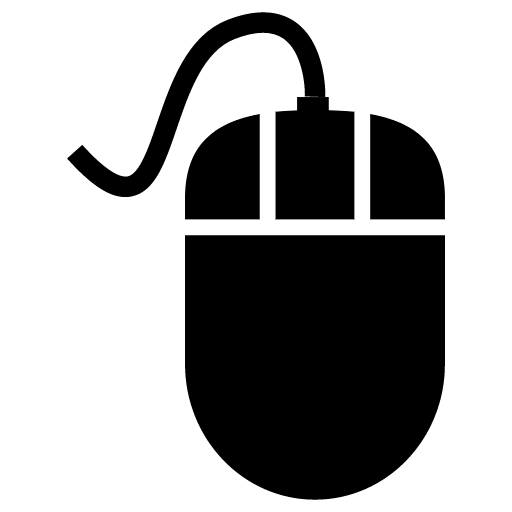
\includegraphics[scale=0.03]{draw_and_tell/fig1/mouse1.png}}
\newcommand*{\iphone}{
\includegraphics[scale=0.06]{draw_and_tell/fig1/microphone.png}}
\newcommand*{\tvbox}[1]{ \begin{turn}{90} \text{#1} \end{turn}}



